\chapter{Experimental Validation and Analysis}
Three different types of experiments were carried out for validating the enhanced D-COACH: i) experiments with simulated teachers for evaluating the learning method under controlled conditions without influence of human factors, ii) validations with real human teachers, and iii) extra validations on real physical systems.

The experiments with the simulated teachers are intended to compare the complete D-COACH presented in Algorithm \ref{algorithm:DeepCOACH}, along with a version of it without buffer (ignoring lines 2 and 11-16), and with a well known DRL agent (Deep Deterministic Policy Gradient DDPG \cite{Lillicrap2015} implemented by OpenAI \cite{baselines}). The comparison is carried out by plotting the cumulative reward obtained at each episode by the agent as a function of time. In the case of D-COACH, the obtained reward is only used as a performance metric. Also, the results are presented as a function of time instead of episodes (except in the Duckie Racing experiment), because episodes can have variable duration depending on the policy. Hence, the episode scale would not properly show the time taken by the learning process, which is an important characteristic, since D-COACH is meant to work with real robots. The simulated environments, Cart-Pole and Car Racing, were ran at $22.5$ and $20.5$ FPS, respectively. These experiments were carried out using human teachers and simulated teachers. Humans had approximately 5 minutes to practice teaching in each environment. The learning curves of agents trained by 10 human teachers were obtained and averaged; the learning curves of agents trained by a simulated teacher were repeated 30 times and averaged. Along with the algebraic mean, the confidence intervals that represent the $60^{th}$ percentile of the data were plotted. In the case of the Car Racing problem, it was observed that coupled training was advantageous when the teachers were humans. The designed coupled signals are shown in Table \ref{table:coupled_car_racing}.

\section{Offline State Learning}
Our proposed algorithm is validated experimentally in three different problems: (i) Cart-Pole (continuous action), which is a simulated task with low-dimensional state space; (ii) Car Racing, a simulated task with high-dimensional state space (raw pixels of an image); and (iii) Duckie Racing, a task with a real robot featuring a high-dimensional state space (raw pixels of an image). 

The experiments with the simulated agents are intended to compare the complete D-COACH presented in Algorithm \ref{algorithm:DeepCOACH}, along with a version of it without buffer (ignoring lines 2 and 11-16), and with a well known DRL agent (Deep Deterministic Policy Gradient DDPG \cite{Lillicrap2015} implemented by OpenAI \cite{baselines}). The comparison is carried out by plotting the cumulative reward obtained at each episode by the agent as a function of time. In the case of D-COACH, the obtained reward is only used as a performance metric. Also, the results are presented as a function of time instead of episodes (except in the Duckie Racing experiment), because episodes can have variable duration depending on the policy. Hence, the episode scale would not properly show the time taken by the learning process, which is an important characteristic, since D-COACH is meant to work with real robots. The simulated environments, Cart-Pole and Car Racing, were ran at $22.5$ and $20.5$ FPS, respectively. These experiments were carried out using human teachers and simulated teachers. Humans had approximately 5 minutes to practice teaching in each environment. The learning curves of agents trained by 10 human teachers were obtained and averaged; the learning curves of agents trained by a simulated teacher were repeated 30 times and averaged. Along with the algebraic mean, the confidence intervals that represent the $60^{th}$ percentile of the data were plotted. In the case of the Car Racing problem, it was observed that coupled training was advantageous when the teachers were humans. The designed coupled signals are shown in Table \ref{table:coupled_car_racing}.

\begin{table}[t]
\centering
\caption{Values of $h$ in the Car Racing problem for human teachers. When feedback is given, the generated correction acts over more than one dimension of the action. For instance, the feedback signal \emph{forward} means that the agent should simultaneously increase its acceleration and decrease its brake.}
\label{table:coupled_car_racing}
\begin{tabular}{lc}
\textbf{Feedback            } & \multicolumn{1}{l}{          }{\textbf{h
(direction, acceleration, brake)}} \\ \hline \hline
Forward     & (0, 1, -1)                                       \\ \hline
Back        & (0, -1, 1)                                       \\ \hline
Left        & (-1, -1, 0)                                      \\ \hline
Right       & (1, -1, 0)                                       \\ \hline
\end{tabular}
\end{table}

The hyper-parameters of the neural networks used in these experiments were tuned with preliminary experiments. Different combinations of them were tested by a human teacher and the ones that made the training easiest were selected (see \figurename~{\ref{fig:network_diagram}}). The D-COACH error magnitude constant $e$ was set to $\textbf{1}$ in this paper.

\subsection{Validation of replay buffer with simulated teachers}
The use of experience replay has been extensively validated in DRL; however, in this approach, we  still consider it necessary to test its impact. Unlike DRL, where the policy is updated with information collected from every time step, in COACH-like methods there only is new data to update the policy when feedback is given by the teacher, so the amount of data used to update the policy may be lower than in the RL case. Since the original COACH has been widely validated with real human teachers in several tasks, we carried out most of the comparisons using  a simulated teacher (a high performance policy standing-in as teacher, which was actually trained with D-COACH and a real human teacher) in this work, like in some of the experiments presented in \cite{Celemin2018AnInteractive}, in order to compare the methods under more controlled conditions. 

The simulated teacher generates feedback using $h = \operatorname{sign}(a_{\mathit{teacher}} - a_{\mathit{agent}})$, whereas the decision of advising feedback at each time step is given by the probability $P_{h} = \alpha \cdot\exp(-\tau\cdot \mathit{timestep})$, where $\{\alpha \in {\rm I\!R}\ | 0 \le \alpha \le 1\}$ and $\{\tau \in {\rm I\!R}\ | 0 \le \tau\}$. Additionally, since human teachers occasionally advise wrong corrections, a probability of giving erroneous feedback $P_{\mathit{err}}$ is added to the model. The variable $P_{\mathit{err}}$ indicates the probability that at least one dimension of $h$ is multiplied by $-1$ when feedback is given.

A comparison of D-COACH with and without the use of an experience replay buffer is carried out by means of the simulated teacher. To test the behavior of these scenarios when erroneous feedback is added, different values of $P_{\mathit{err}}$ are selected. These results can be seen in \figurename~{\ref{fig:buffer_cart_pole}} and \figurename~{\ref{fig:buffer_car_racing}} (for better readability, no confidence intervals were added).

\begin{figure}[t]
    \centering
    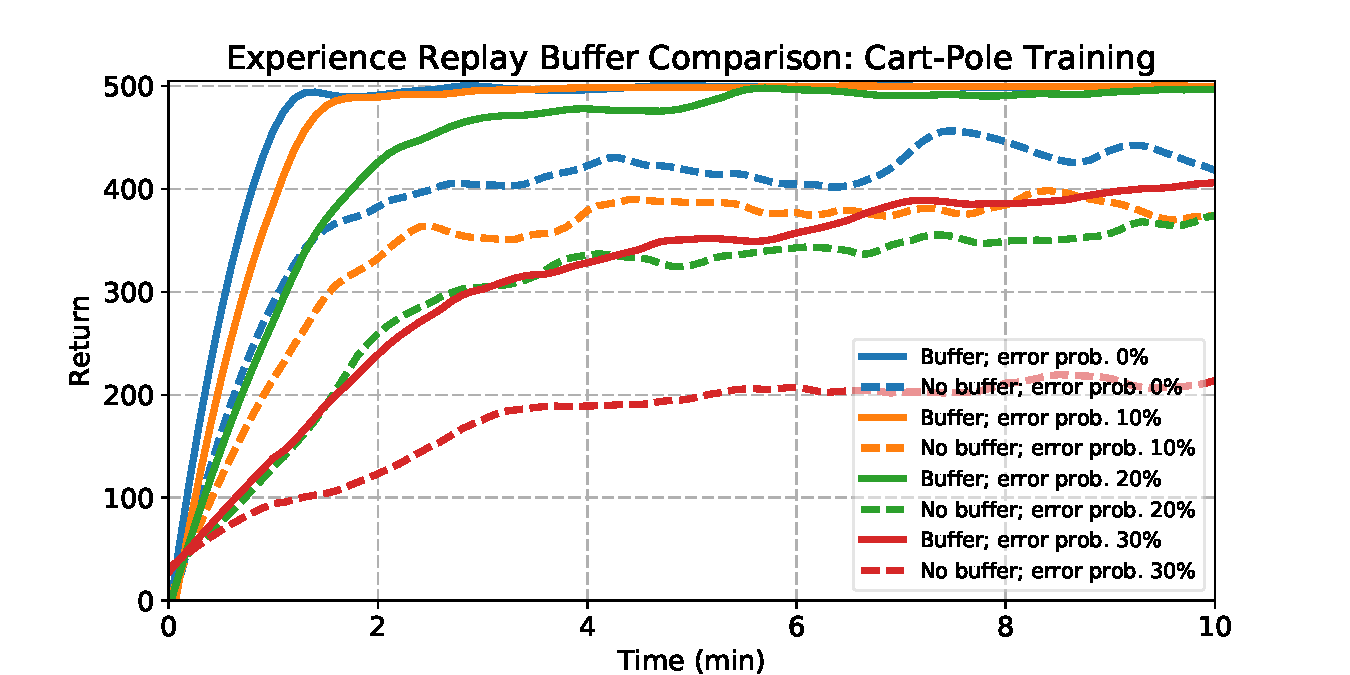
\includegraphics[width=0.9\linewidth]{imagenes/cap3/buffer_cart_pole.pdf}
    \caption{Comparison between using or not experience replay buffer for different values of $P_\mathit{err}$ in the Cart-Pole problem. Buffer: $K = 200$; $b = 10$; $N = 50$. $P_{h}$: $\alpha = 0.6$; $\tau = 0.0003$. Simulated teacher network learning rate: $0.0003$.}
    \label{fig:buffer_cart_pole}
\end{figure}

\begin{figure}[t]
    \centering
    \vspace{-0.2cm}
    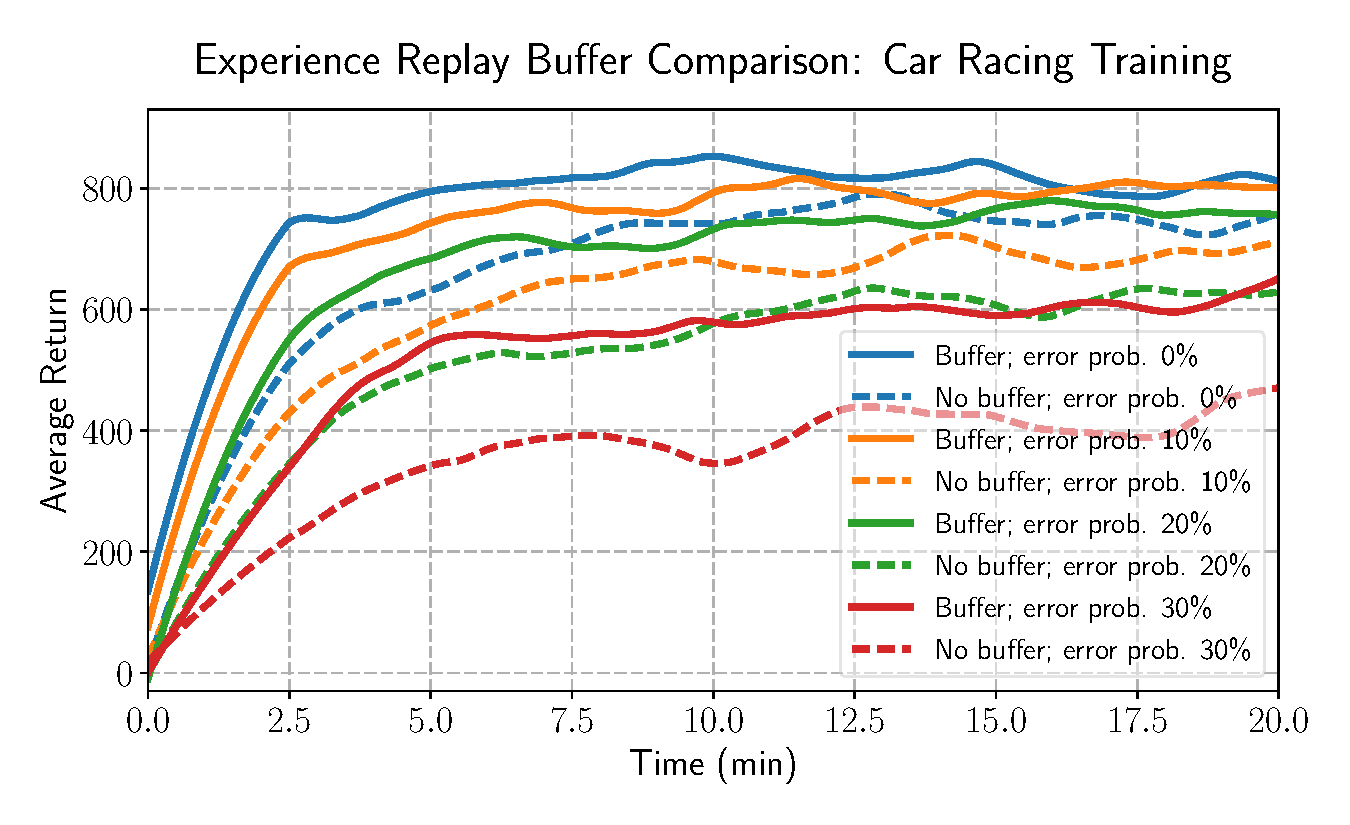
\includegraphics[width=0.9\linewidth]{imagenes/cap3/bufferCarRacing.pdf}
    \vspace{-0.2cm}
    \caption{Comparison between using or not experience replay buffer for different values of $P_\mathit{err}$ in the CarRacing problem. Buffer: $K = 1000$; $b = 10$; $N = 100$. $P_{h}$: $\alpha = 0.6$; $\tau = 0.000015$. Simulated teacher network learning rate: $0.0003$.}
    \label{fig:buffer_car_racing}
\end{figure}

In \figurename~{\ref{fig:buffer_cart_pole}} and \figurename~{\ref{fig:buffer_car_racing}} the learning curves show a large difference between the processes of learning that use experience replay buffer with respect to the cases without the buffer. In the case without the buffer, which is more similar to the original COACH, it is possible to see that the learning agent is not benefiting from the advised corrections as much as it can do when the pieces of advice are kept in the memory. For instance, we can see that D-COACH learns more from corrections with $20 \%$ of mistakes when using the buffer than in the case of perfect corrections, but without any buffering. This means the buffer is necessary for increasing the use of the information available, even when this information is corrupted and not clean.

\subsection{Comparison of DRL and D-COACH using real human teachers}
\begin{figure}[t]
    \centering
    \vspace{-0.2cm}
    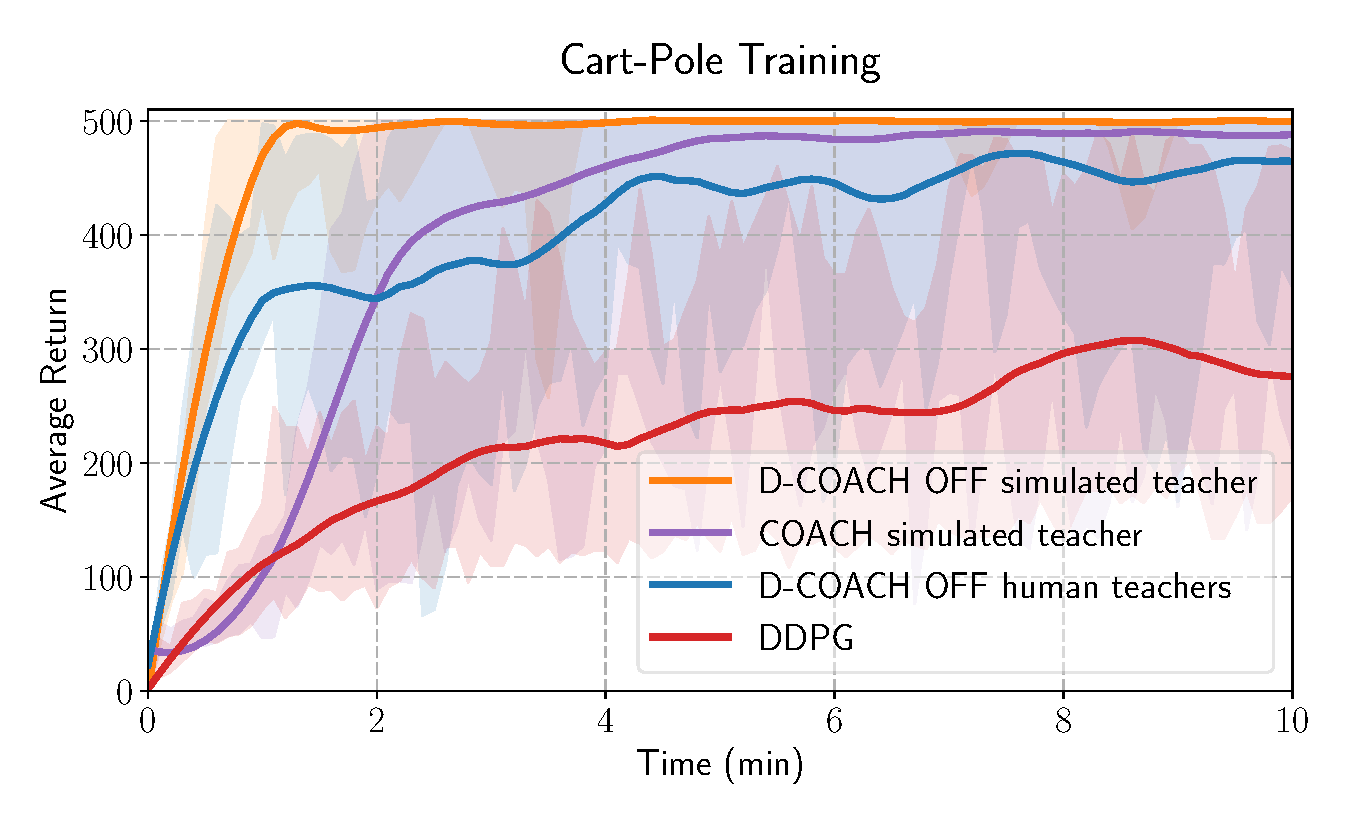
\includegraphics[width=0.9\linewidth]{imagenes/cap3/offline_cart_pole_humans.pdf}
    \vspace{-0.2cm}
    \caption{Cart-Pole training. Buffer: $K = 200$; $b = 10$; $N = 50$. $P_{h}$: $\alpha = 0.6$; $\tau = 0.0003$. Human teacher network learning rate: $0.003$; Simulated teacher network learning rate: $0.0003$.}
    \label{fig:cartpole_results}
\end{figure}

These experiments are intended to compare the learning process of D-COACH (simulated teacher and human teacher) with the DRL algorithm DDPG. Taking into account that the Cart-Pole problem has a low dimensional state space, the original COACH, based on basis functions, is also included in the comparison. In this case, $P_\mathit{err}=0\%$ was used for the simulated teachers. The results of this problem are shown in \figurename~{\ref{fig:cartpole_results}}, wherein it is possible to see that COACH-like methods outperform the DRL agent with a large difference. When using the simulated teacher, D-COACH learns faster than the original COACH. The performance of D-COACH with human teachers decreases with respect to the simulated teacher. This is because human teachers are not perfect and make mistakes, but they are being compared with a simulated teacher with $P_\mathit{err}=0\%$, which means that it makes no mistakes. Also because the simulated teacher model is quite simple to represent the complexity of the human behavior, then, although it is not very realistic, it is still useful for comparisons of interactive learning strategies under similar conditions.

In \figurename~{\ref{fig:racing_car_results}} the learning curves of the Car Racing problem are presented. Again, D-COACH results in a fast convergence. Unlike reported results of DRL algorithms for this problem, in the very early minutes D-COACH reaches high performance policies that have not been obtained by most of the DRL approaches, to the best of our knowledge. If we compare a policy trained with D-COACH for approximately 75 minutes by an experienced teacher against several state-of-the-art DRL approaches, it can be seen that it outperforms most of them (see Table \ref{CarRacing_table}). The problem is considered to be solved if the agent gets an average score of 900 or more over 100 random tracks. However, we observed that this value can substantially vary between different evaluations, so in Table \ref{CarRacing_table}, the obtained range of values over 20 evaluations is presented for D-COACH.
\vspace{-0.4cm}

\begin{figure}[t]
    \centering
    \vspace{-0.2cm}
    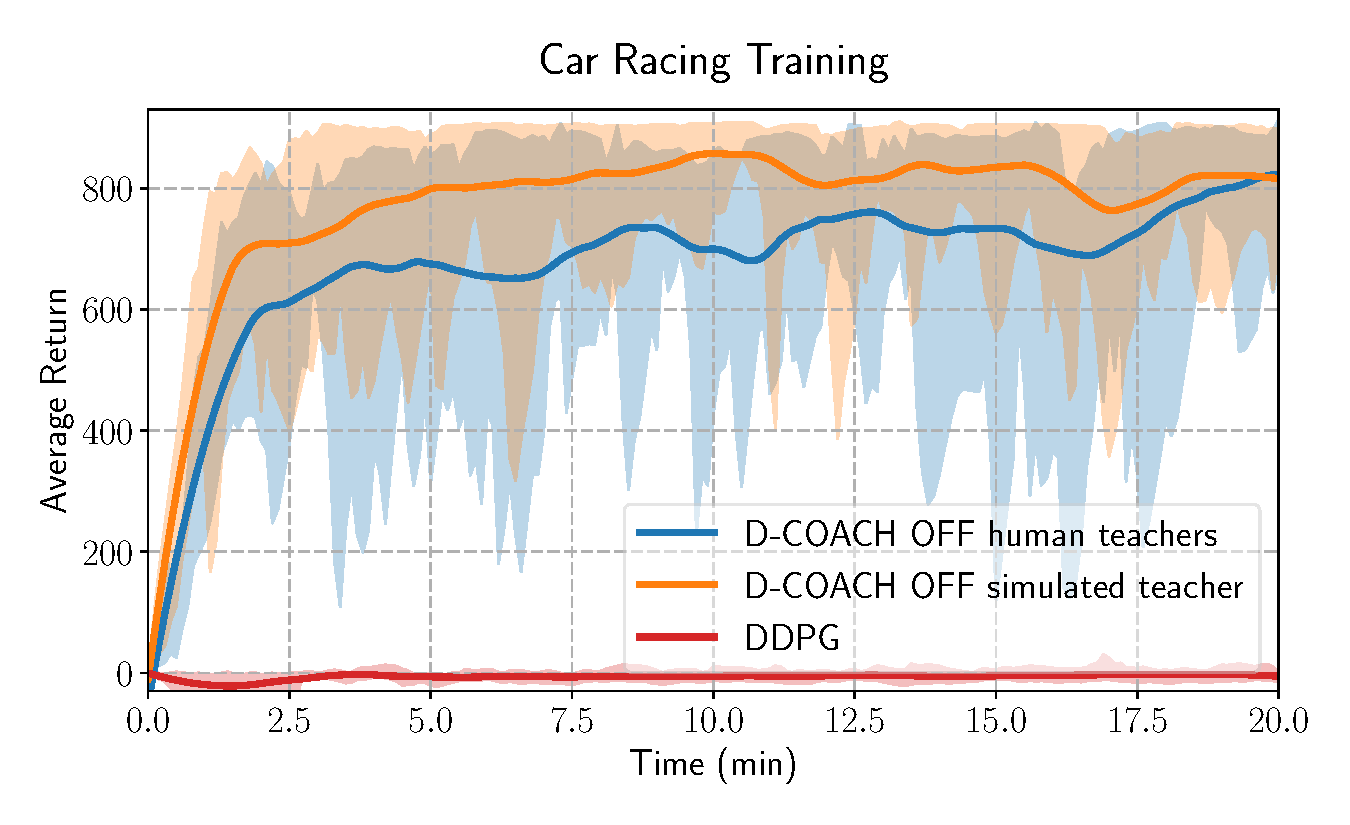
\includegraphics[width=0.9\linewidth]{imagenes/cap3/offline_car_racing_humans.pdf}
    \vspace{-0.2cm}
    \caption{Racing Car training. Buffer: $K = 1000$; $b = 10$; $N = 100$. $P_{h}$: $\alpha = 0.6$; $\tau = 0.000015$. Human teacher network learning rate: $0.001$; Simulated teacher network learning rate: $0.0003$.}
    \label{fig:racing_car_results}
\end{figure}

\begin{table}[t]
\centering
\caption{Car Racing state-of-the-art learning algorithms comparison. DRL results taken from \cite{Ha2018}.}
\label{CarRacing_table}
\begin{tabular}{lc}
\multicolumn{1}{c}{\textbf{Method}}      & \multicolumn{1}{l}{\textbf{Average Score over 100 Random Tracks}} \\ \hline\hline
DQN                                      & 343 $\pm$ 18                                                      \\ \hline
A3C (continuous)                         & 591 $\pm$ 45                                                      \\ \hline
A3C (discrete)                           & 652 $\pm$ 10                                                      \\ \hline
ceobillionaire’s algorithm (unpublished) & 838 $\pm$ 11                                                      \\ \hline
Full World Model                         & 906 $\pm$ 21                                                      \\ \hline
\textbf{D-COACH (experienced teacher)}                         & \textbf{895 - 909 $\pm$ 18 - 80} \\
& \textbf{Average over 20 evaluations: 903 $\pm$ 46}
\\ \hline
\end{tabular}
\end{table}

\subsection{Validation in a real system}
In the third problem that we called Duckie Racing, an agent has to learn to drive a Duckiebot (from the project  Duckietown \cite{Paull2017} with modifications from the Chile Duckietown Team\footnote{\url{https://github.com/Duckietown-Chile/}}) autonomously through a track based on raw visual information of an onboard camera. The actions in this problem are the forward velocity and the steering angle of the Duckiebot. Two tasks are set for this environment: (i) driving the Duckiebot freely through the track, with permission to drive in both lanes, and (ii) driving the Duckiebot only in the right lane, which demands more accuracy in driving. In this problem, an episode stops if the robot leaves the track/right lane, or after 30 seconds. The performance index in this task is the percentage of the total track length traveled during the episode. Hence the faster and more accurate the Duckiebot drives, the more distance it will travel.

This problem is not used for comparisons of the methods, but only as a validation of D-COACH using experience replay, which showed to be the best alternative in the previous problems. \figurename~\ref{fig:racing_duckie_results} shows the learning curve for each of the tasks explored in this environment with a real robot and a real human teacher. The curves and the video\footnote{https://youtu.be/vcEtuRrRIe4} attached to this paper show that the system quickly learns to drive properly through the road based only on the human corrections. As expected, the policy is faster when the robot has the freedom to drive over both lanes. Learning this task with RL would definitely take more training time, and might need an external perception system to compute the reward function, whereas with D-COACH this performance index does not have any influence on the learning process, rather it is used for descriptive and comparative purposes.

\begin{figure}[H]
    \centering
    \begin{minipage}{.5\textwidth}
    \vspace{-0.2cm}
    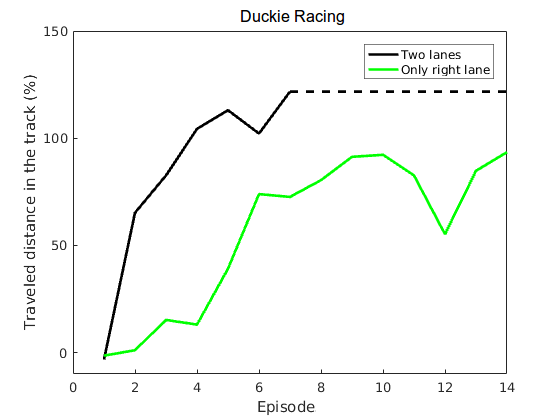
\includegraphics[width=1.0\linewidth]{imagenes/cap3/racing_duckie_results.png}
    \vspace{-0.2cm}
    \caption{Duckie Racing training.}
    \label{fig:racing_duckie_results}
    \end{minipage}%
    \begin{minipage}{.5\textwidth}
    \centering
    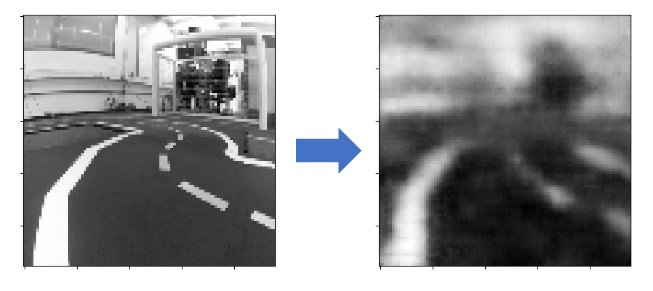
\includegraphics[width=1.0\linewidth]{imagenes/cap3/AE_duckie2.png}
    \vspace{-0.2cm}
    \caption{Duckie Racing autoencoder input (left) vs output (right).}
    \label{fig:AE_duckie}
    \end{minipage}
\end{figure}

\section{Online State Learning}
Three different types of experiments were carried out for validating the enhanced D-COACH: i) experiments with simulated teachers for evaluating the learning method under controlled conditions without influence of human factors, ii) validations with real human teachers, and iii) extra validations on real physical systems.

In these experiments we denote the enhanced D-COACH simply with `D-COACH', while we from now on we call the previous version `basic D-COACH'. In the experiments, the learning processes are analyzed in three different problems:

\textbf{Car Racing:} a simulated problem (from OpenAI gym \cite{brockman2016openai}) in which the agent has to learn to drive from a top-down view of a racing car game (see Figure \ref{fig:Car_Racing}). The objective of the task is to drive a racetrack as fast as possible without leaving it. The default state that is given by the environment is a $96\times96\times3$ top-down view of the car which we downsampled to $64\times64\times1$. The continuous action space consists of 3 dimensions: \textbf{[direction, acceleration, brake]}. The \emph{direction} range goes from $-1$ to $1$, the \emph{acceleration} from $0$ to $1$ and the \emph{brake} from $0$ to $1$. In this problem, experiments with the simulated teacher and human teachers were carried out. The coupled feedback strategy was used in the experiments with human teachers, as it is presented \cite{perez2018interactive}.

\begin{figure}[h]
    \centering
    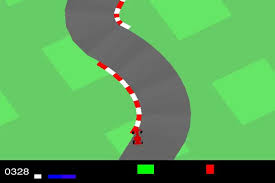
\includegraphics[scale=0.8]{imagenes/cap3/car_racing_env.jpg}
    \caption{Car Racing, environment view.}
    \label{fig:Car_Racing}
\end{figure}
    
\textbf{Duckie Racing:} This is also a driving task, but in this case with a real/simulated robot which has an onboard camera, that gives a first-person view of the environment. The real robot consist of a Duckiebot from the project Duckietown \cite{Paull2017}. The simulated robot is based on \cite{gym_duckietown}. A $120\times160\times3$ observation image is received from the environment which is downsampled to $64\times64\times1$. The same road was used for both the simulated and real robot. In the simulations, at the start of each episode, the robot can start, randomly, at the points A or B (plus random noise) of the map (see Figure \ref{fig:duckietown}). Each simulated episode lasts 1000 episodes (unless the robot leaves the road before) and as a performance metric a modified version of the default reward function of the environment is used, which has the following shape: $R = Av\theta - Bd$. $A$ and $B$ are constants ($A=100$, $B=1$), $v$ is the linear velocity of the duckiebot, $\theta$ is its orientation with respect to $C$ (a bezier curve that defines the path the agent is expected to follow) and $d$ is its distance to $C$. The duckiebot is a differential robot, so the default actions consisted of speed commands ranging from -1 to 1 for each of the two wheels. To make it more intuitive for a human teacher to give feedback, an inverse kinematics module was added to the environment for the actions to be linear and rotational speeds instead, also ranging from -1 to 1. This problem is also used for experiments and validation with simulated and real human teachers.

\begin{figure}[h]
\centering
\subfloat[][Duckiebot.]{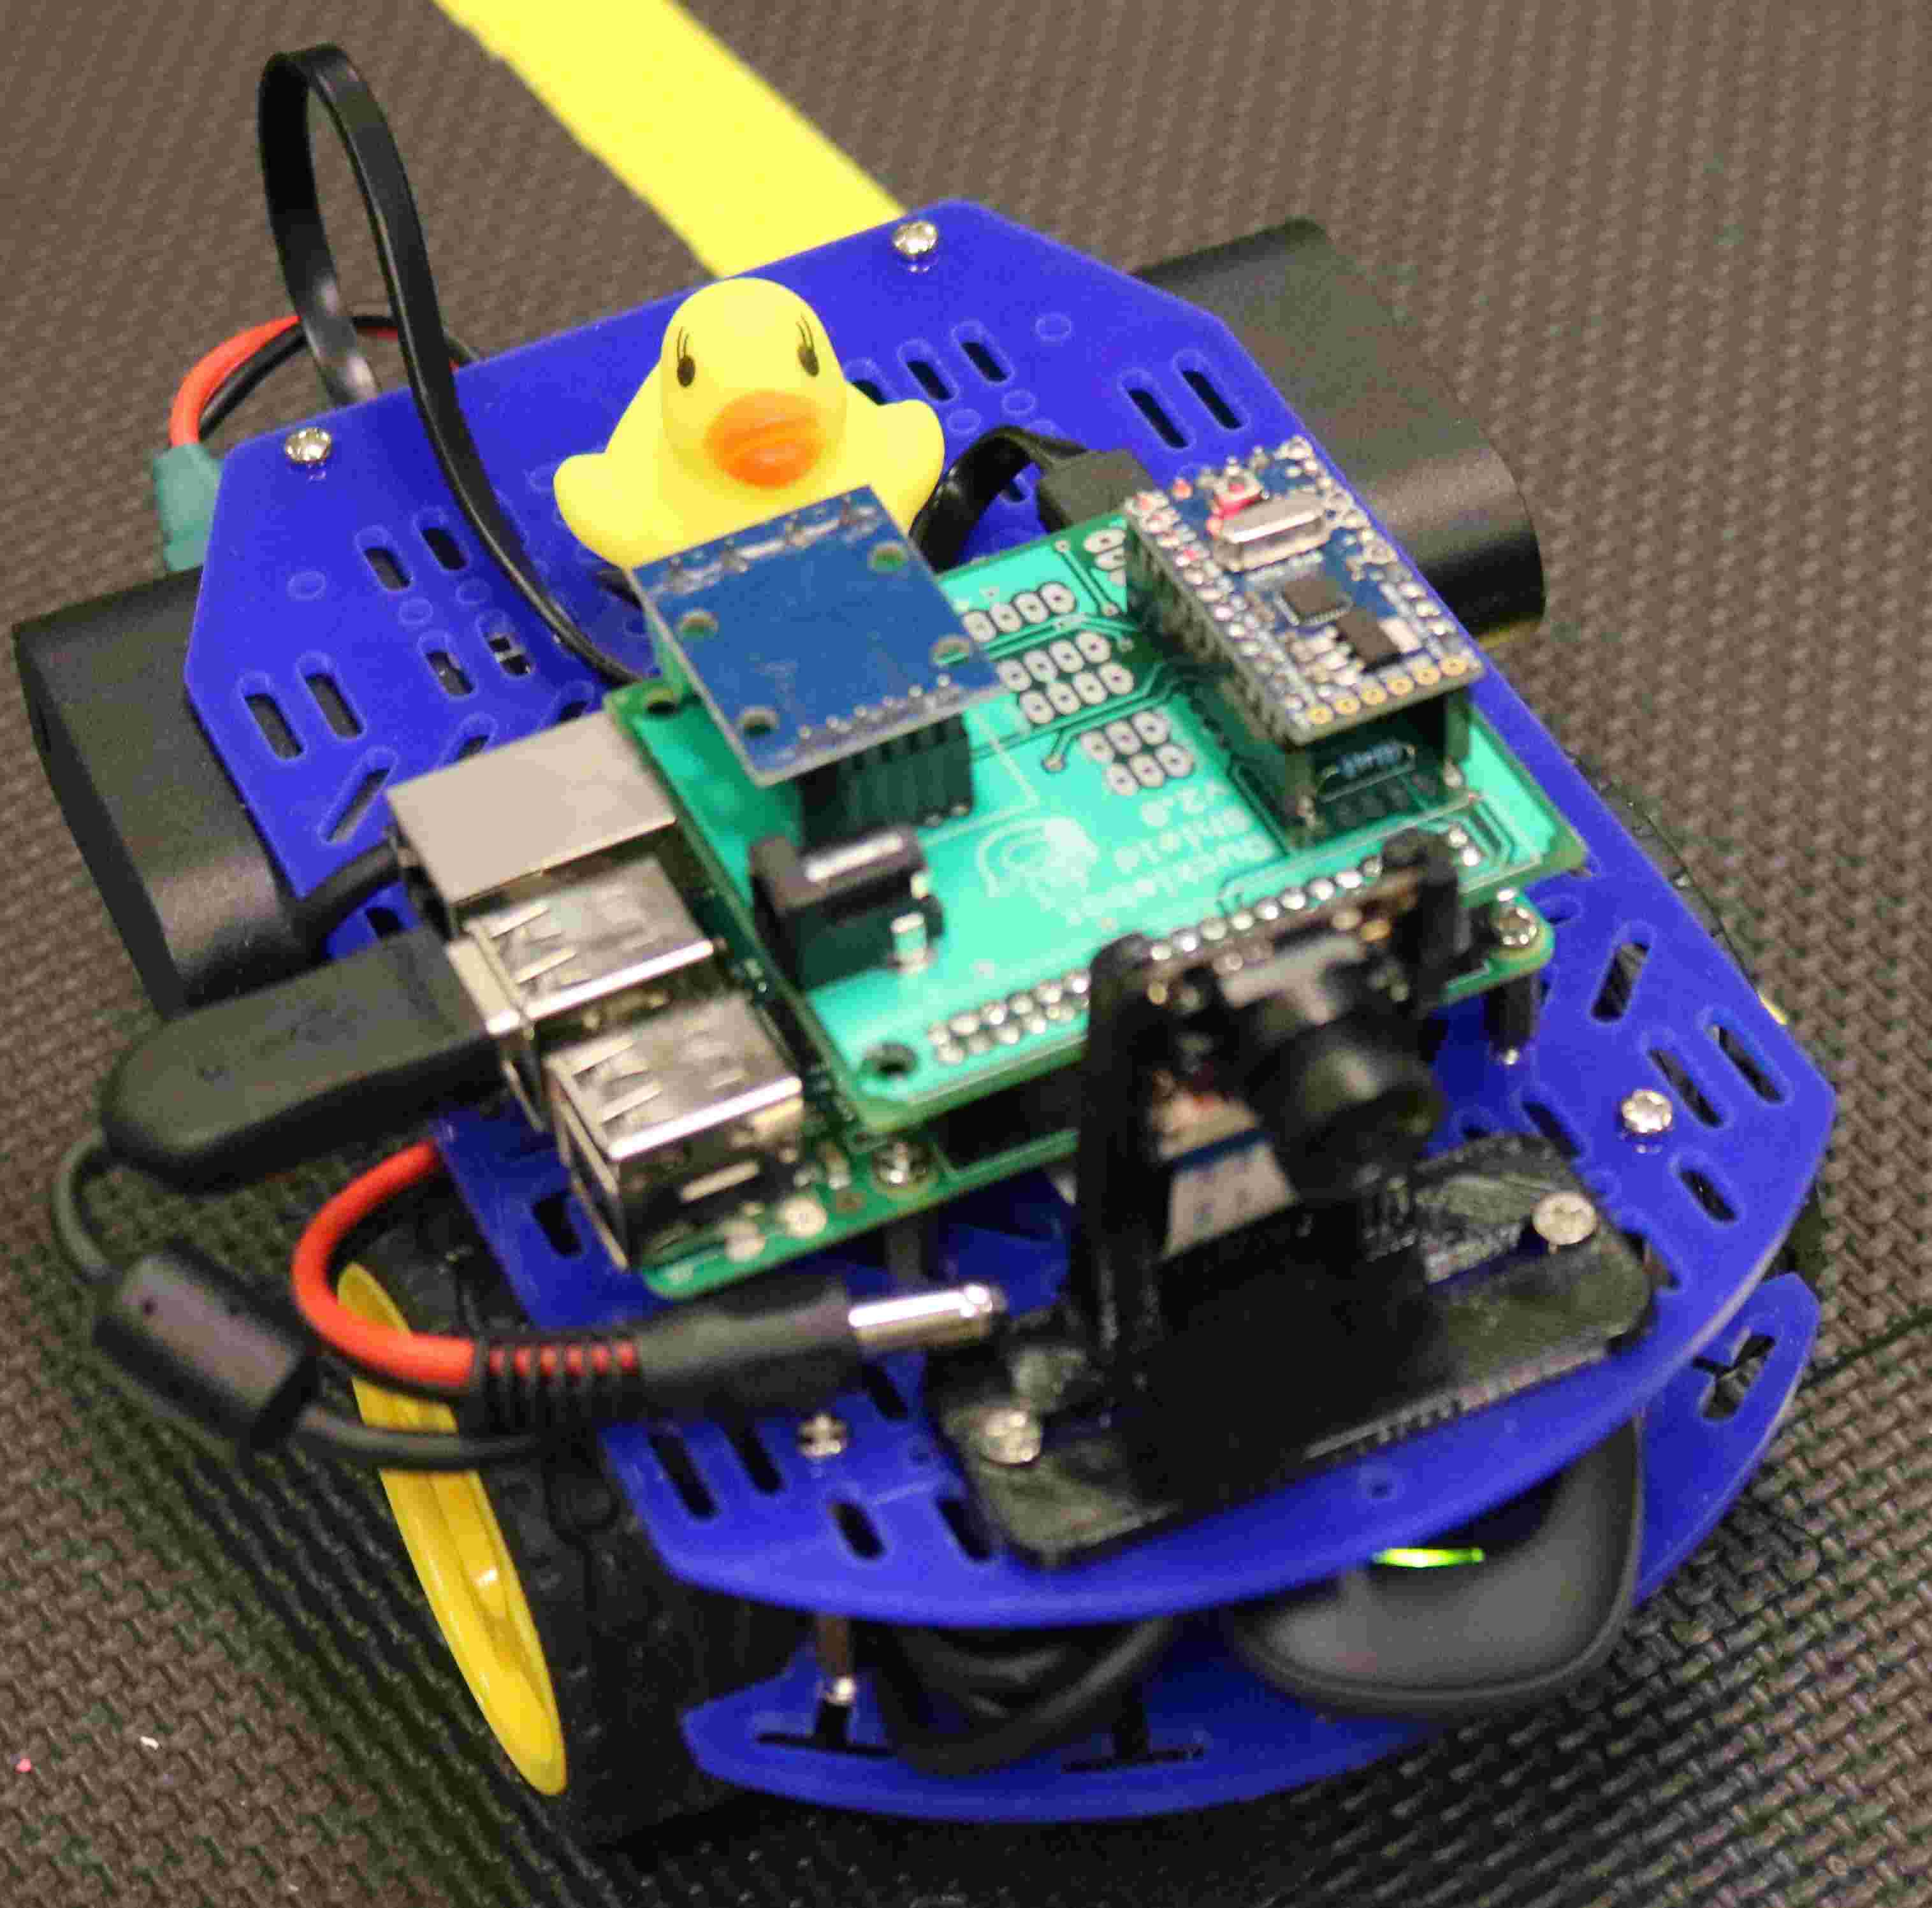
\includegraphics[width=0.305\linewidth]{imagenes/cap3/duckie_image.jpg}} 
\hspace{1.3cm}
\subfloat[][First-person view.]{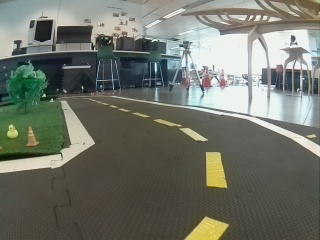
\includegraphics[width=0.4\linewidth]{imagenes/cap3/real_duckie_view.jpg}}
\hspace{2cm}
\subfloat[][Map.]{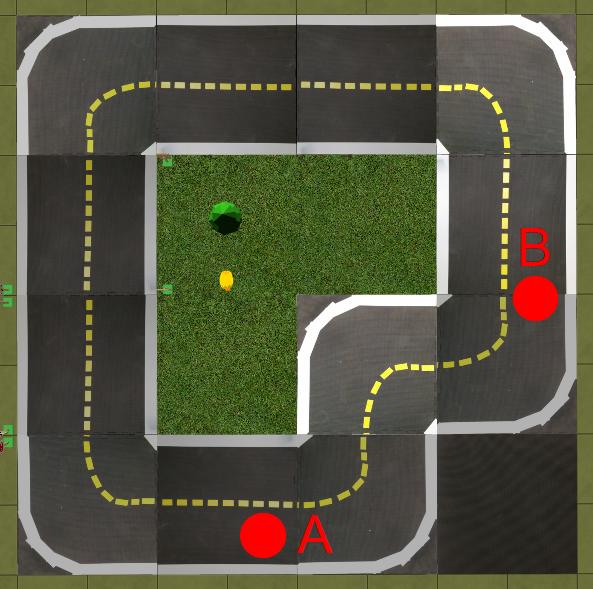
\includegraphics[width=0.305\linewidth]{imagenes/cap3/duckie_map.png}}
\hspace{1.3cm}
\subfloat[][First-person simulated view.]{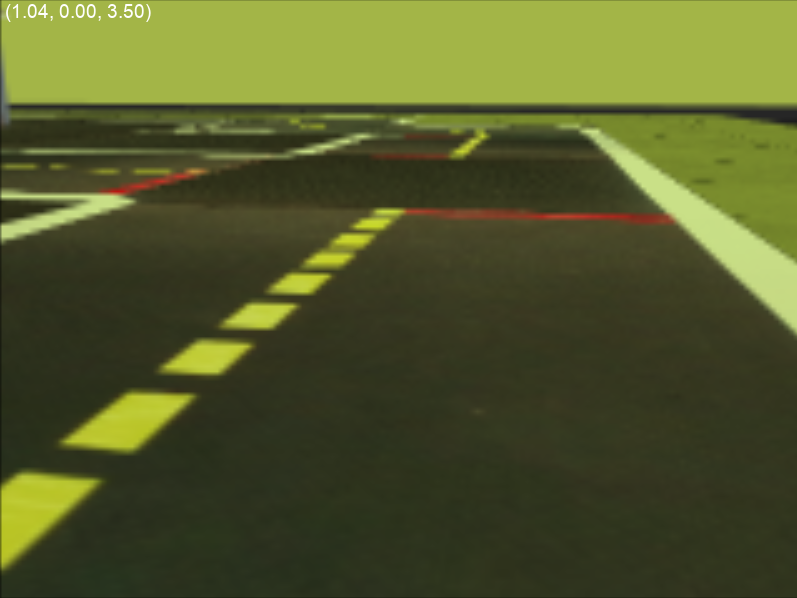
\includegraphics[width=0.4\linewidth]{imagenes/cap3/simplesim_1.png}}
\caption{Duckietown.} 
\label{fig:duckietown2} 
\end{figure}

\textbf{Pusher/Reacher:}. Two validation tasks with a 3DoF robotic arm (see Figure \ref{fig:PusherReacher}). The problems of pushing  and reaching an object were addressed.  
For both tasks the robot arm is placed in front of the work-space and an RGB camera is fixed overhead for capturing the top-down view of the environment with images of $640\times480\times3$ size. The images are downsampled to $64\times64\times3$. The objective of the Pusher task is to move the object placed in the work-space down, until it is out, as depicted in Figure \ref{fig:PusherReacher}(b). The objective of the Reacher is to track the position of the object with the arm's end effector (Figure \ref{fig:PusherReacher}(c)). The experiments of the tasks with the 3DoF robot arm were intended only to validate the proposed learning method in another real setup, no comparisons were carried out.

All the results that present averaged data in the form of a curve have confidence intervals that represent the $60^{th}$ percentile of the data.

The neural network hyperparameters proposed in \cite{perez2018interactive} were used in this work.  

\begin{figure}[t]
\centering
\subfloat[][3DoF robot arm.]{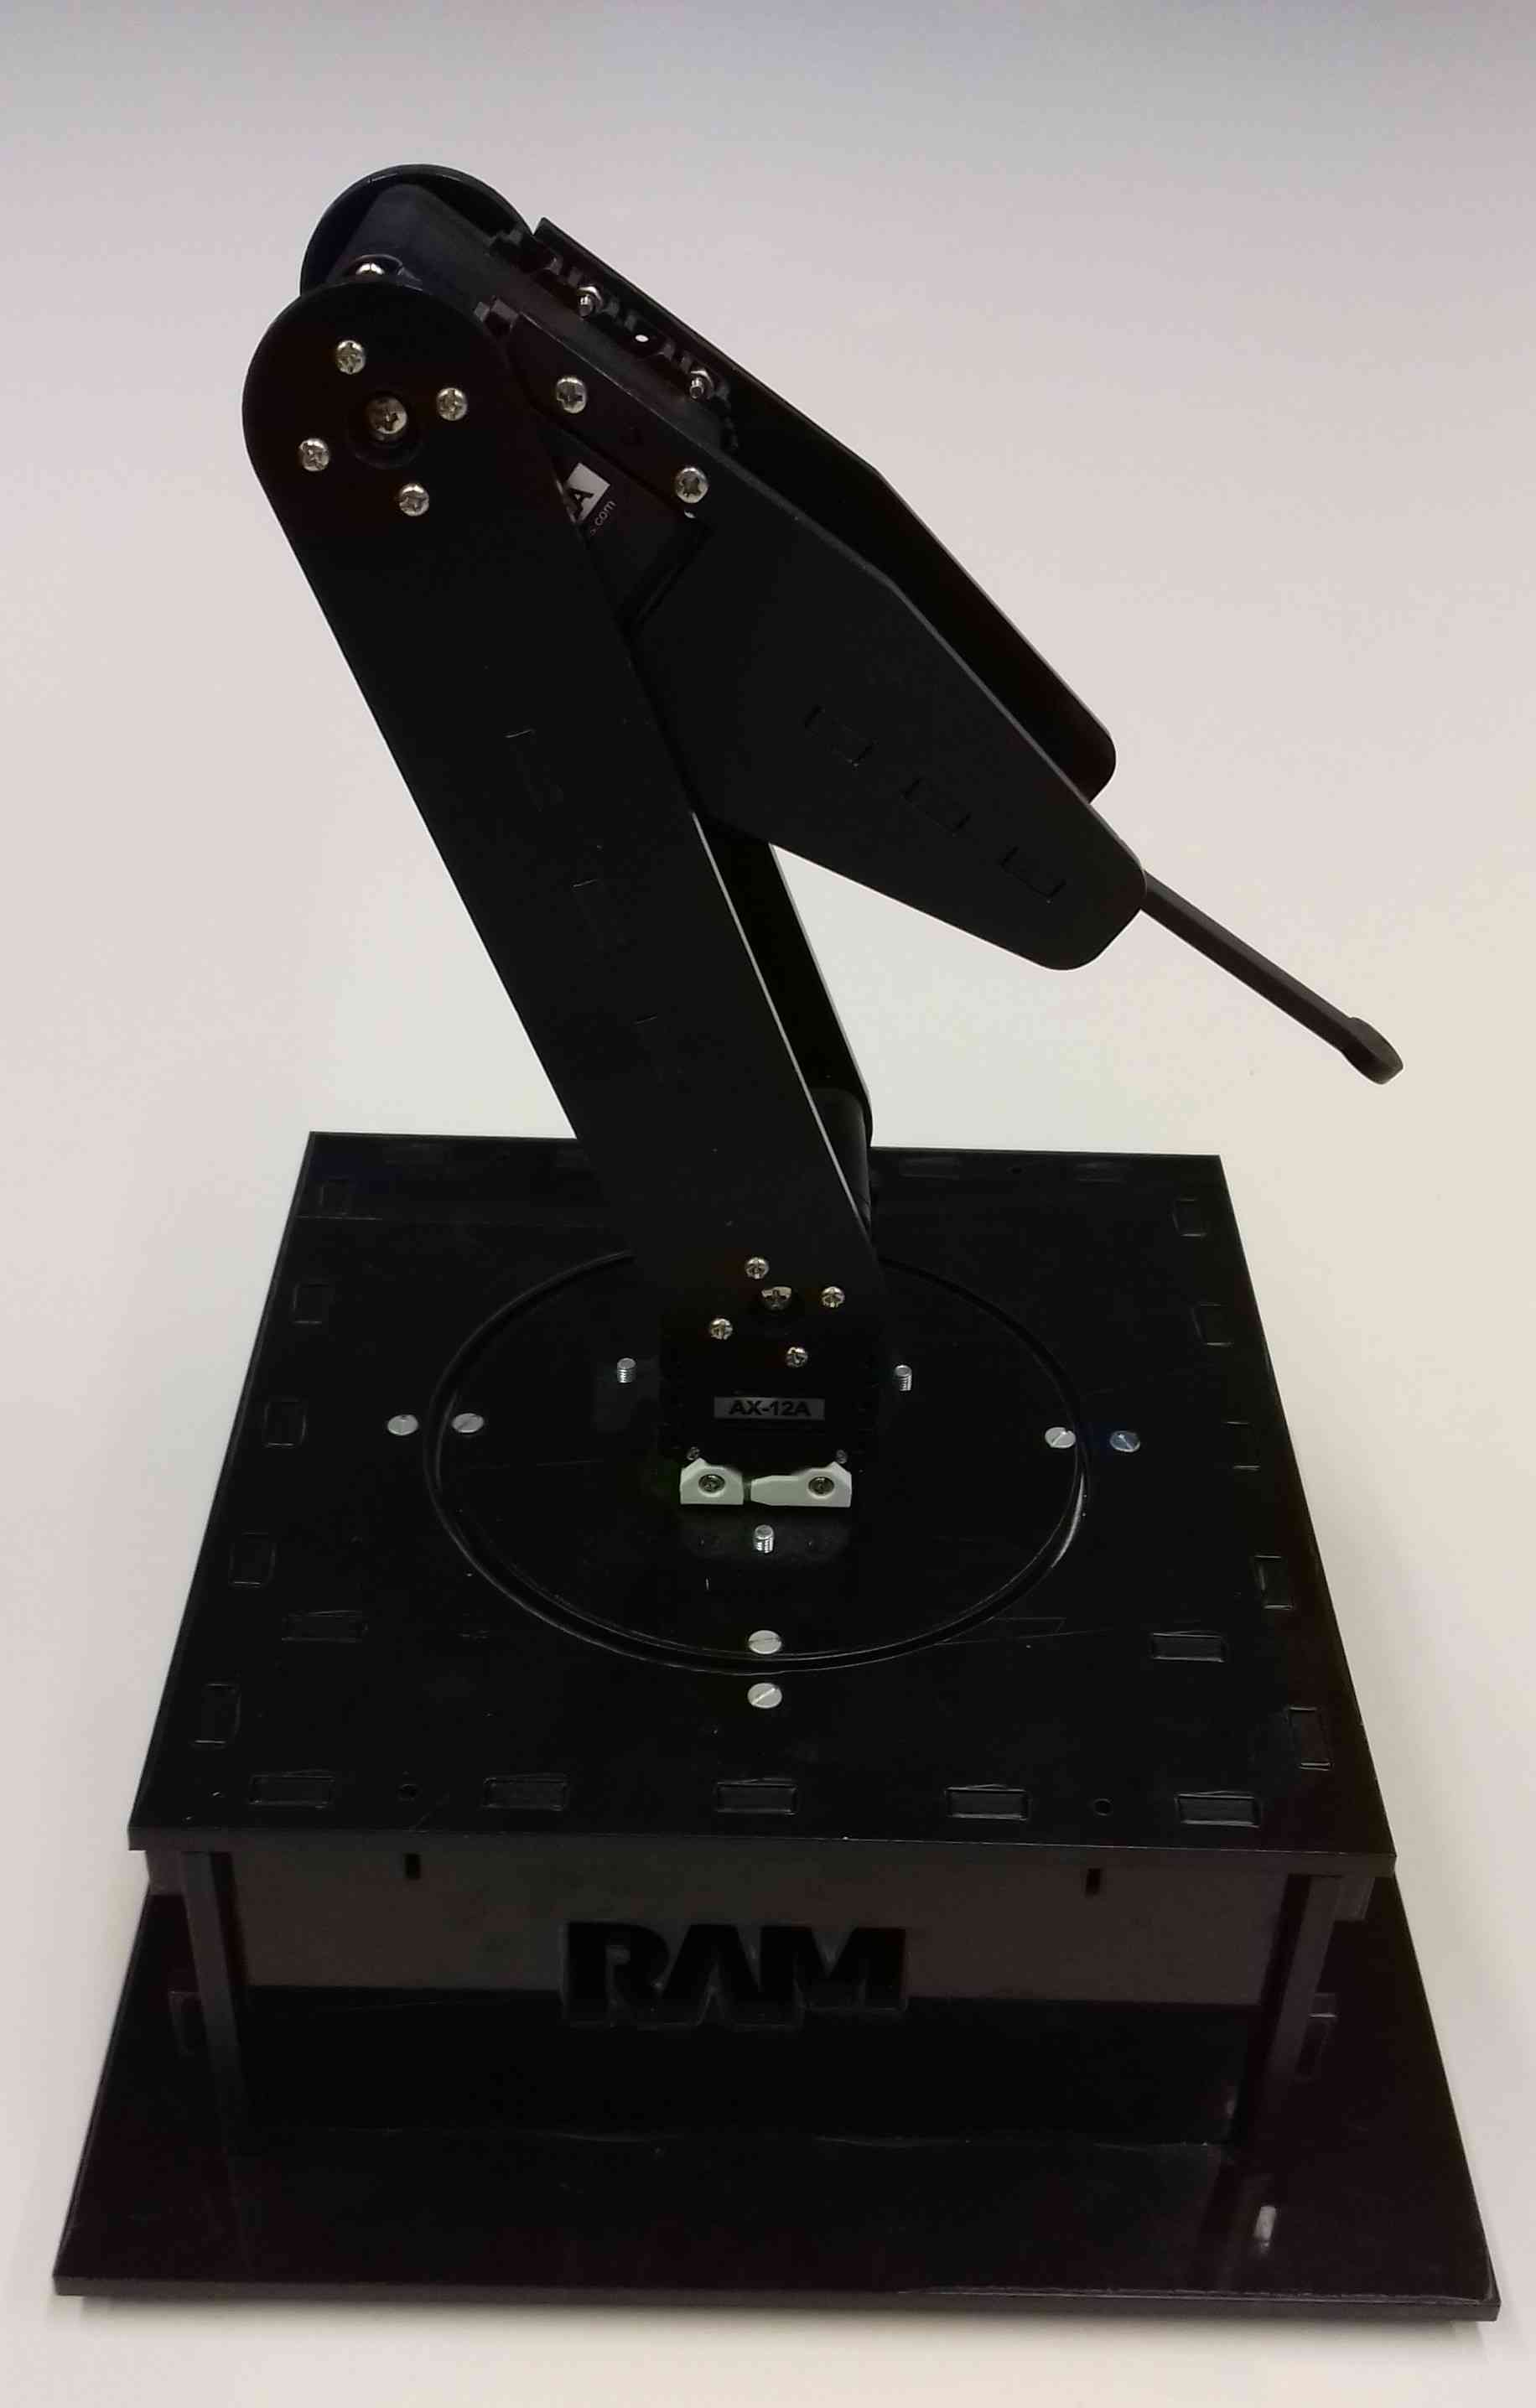
\includegraphics[width=0.2\linewidth]{imagenes/cap3/3dofarm2.jpg}} 
\hspace{0.25cm}
\subfloat[][Pusher task.]{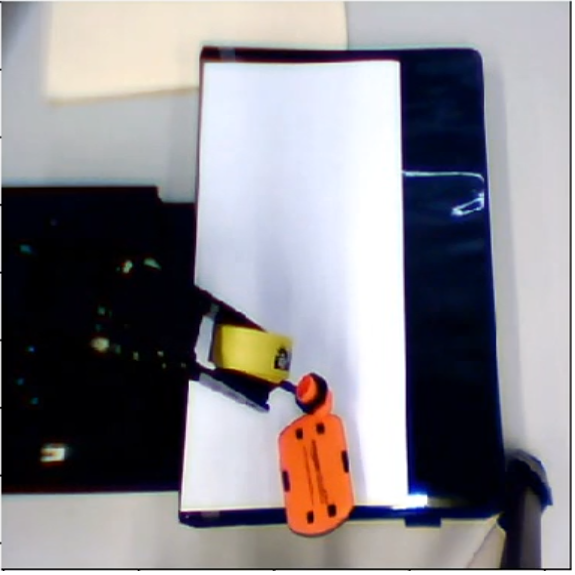
\includegraphics[width=0.315\linewidth]{imagenes/cap3/pusher.png}} 
\hspace{0.25cm}
\subfloat[][Reacher task.]{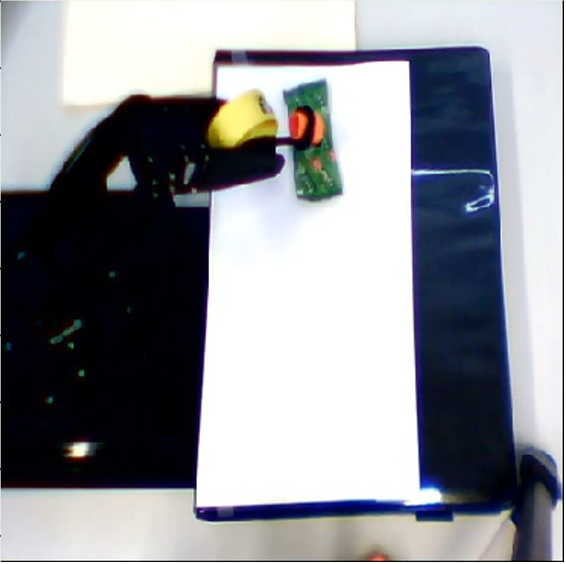
\includegraphics[width=0.315\linewidth]{imagenes/cap3/reacher.png}}
\hspace{0.25cm}
\caption{Pusher/Reacher.} 
\label{fig:PusherReacher} 
\end{figure}


\subsection{Study with Simulated teacher}
In order to evaluate the method along with subtle variants under more controlled conditions, a high performance policy standing-in as a teacher, which was actually trained with D-COACH and a real human teacher, was used (similar approach to the one used in  \cite{Celemin2018AnInteractive}). The simulated teacher generates feedback computing $h = \operatorname{sign}(a_{teacher} - a_{agent})$, whereas the decision on whether to provide feedback at each time step is given by the probability $P_{h} = \alpha \cdot\exp(-\tau\cdot episode)$, where $\{\alpha \in {\rm I\!R}\ | 0 \le \alpha \le 1\}$ and $\{\tau \in {\rm I\!R}\ | 0 \le \tau\}$. The learning curves were repeated 30 times and averaged.

In order to perform an ablation study that evaluates the contribution of the new components of the enhanced D-COACH, the complete method (Algorithm \ref{algorithm:DeepCOACH}) is compared to a second variant that does not include the AE contribution, and learns the whole policy network only with the cost of predicting the action (ignoring lines 17-21). This variant  works like the basic D-COACH proposed in \cite{perez2018interactive}, but skipping the first two steps of recording demonstrations and pre-training the AE, i.e. learning from scratch, which means that the convolutional layers are also learned with the teacher's corrections.

The third evaluated variant includes the AE cost function, but never freezes the convolutional layers, so it always modifies the parameters of the complete policy network using the gradient of both cost functions (i.e. setting $\epsilon=0$ for the condition in line 17). The learning curves of the three cases of D-COACH are compared against the baseline one of a DDPG-based RL agent \cite{Lillicrap2015}, using the OpenAI implementation \cite{baselines}. The curves are the average of 30 runs for each case, showing the evolution of the return through the learning time. The time considered is measured when rendering the environments, i.e. no environment acceleration, since D-COACH is intended for learning with real systems wherein speeding up the environment is not possible.

\begin{figure}[h]
    \centering
    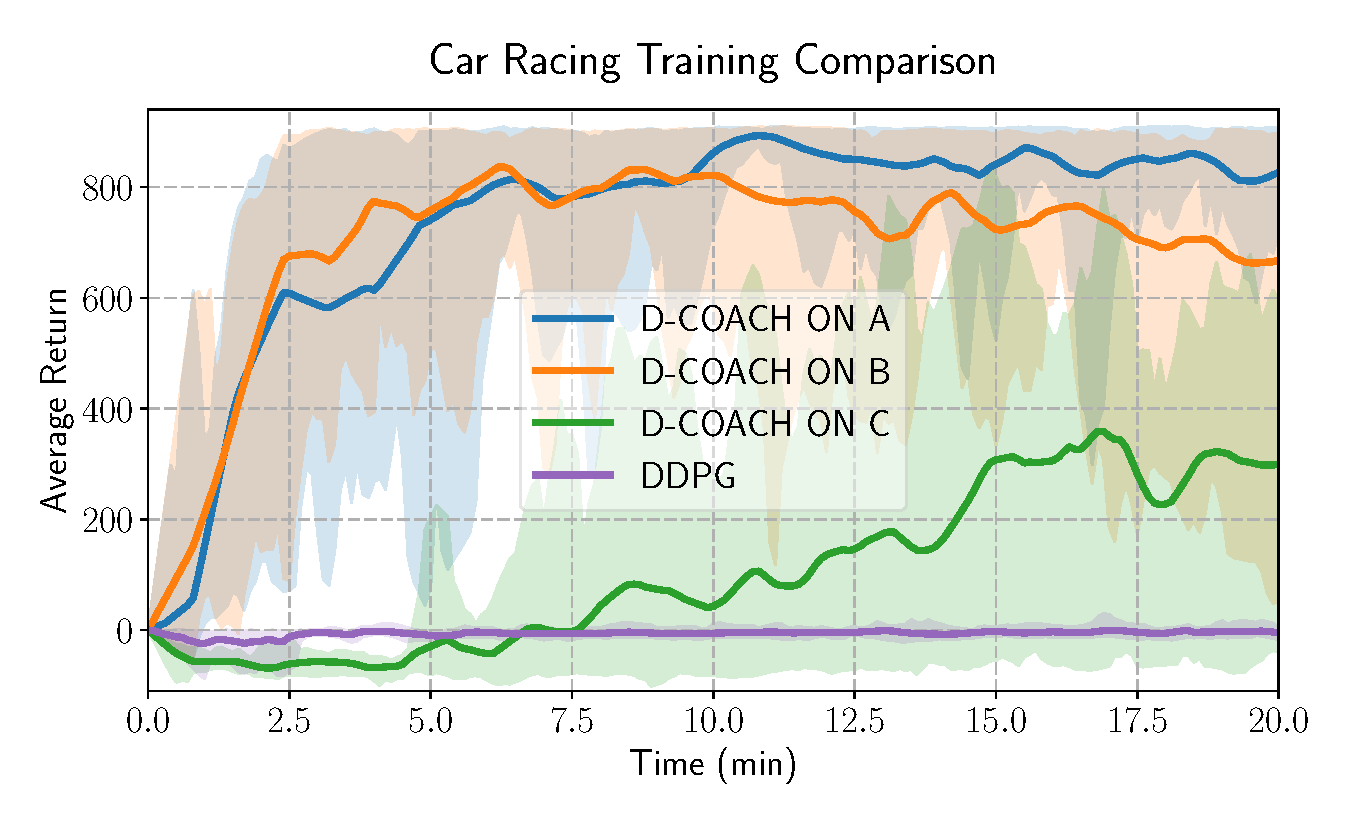
\includegraphics[width=0.9\linewidth]{imagenes/cap3/car_racing_sim_ICRA.pdf}
    \caption{Car Racing results for simulated teacher with D-COACH and DDPG. D-COACH A: policy and AE costs, freezing conv. layers; D-COACH B: policy and AE costs; D-COACH C: only policy cost. Buffer: $K = 1000$; $b = 10$; $N = 8$. $P_{h}$: $\alpha = 0.6$; $\tau = 0.000015$.}
    \label{fig:racing_car_results}
\end{figure}

\begin{figure}[h]
    \centering
    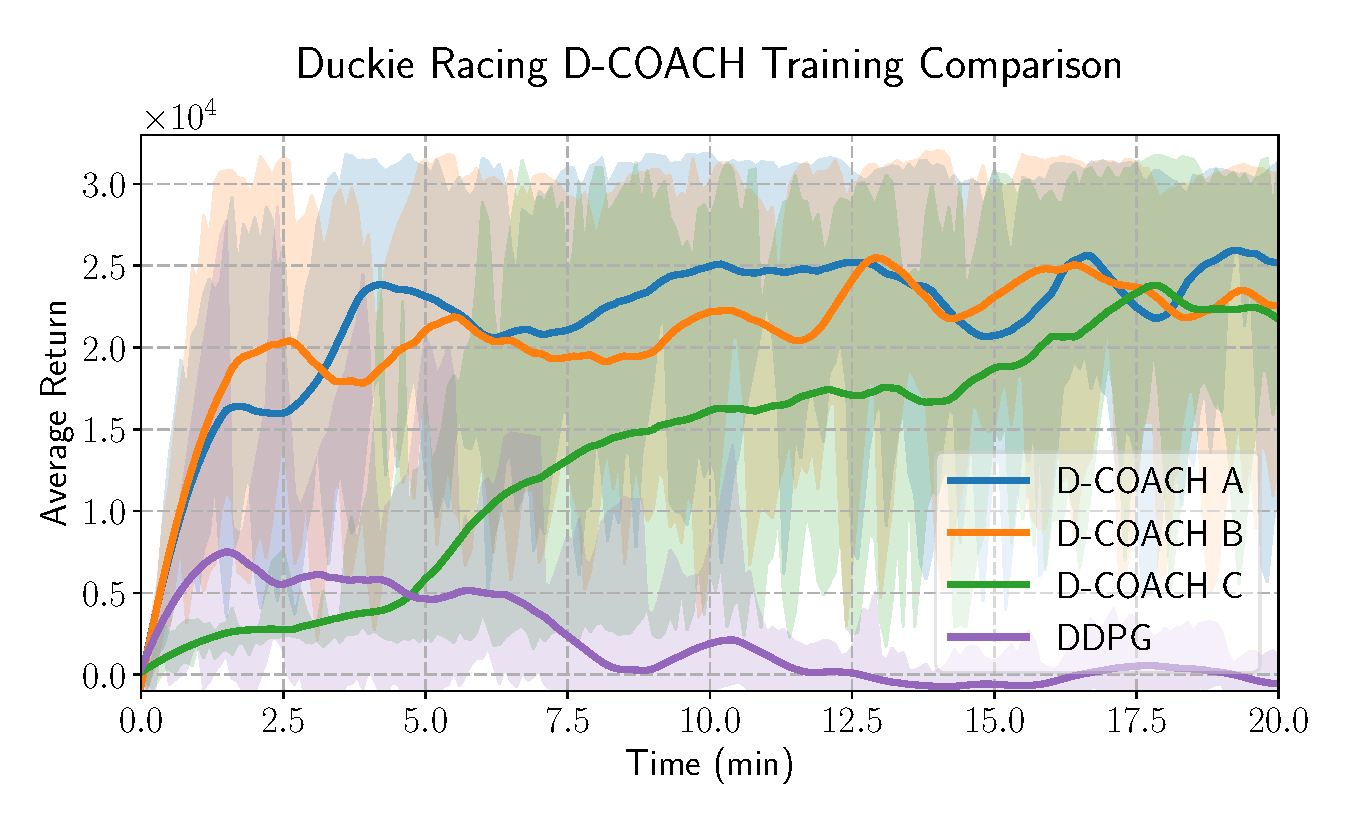
\includegraphics[width=0.9\linewidth]{imagenes/cap3/duckie_sim_ICRA.pdf}
    \caption{Duckie Racing results for simulated teacher with D-COACH and DDPG. D-COACH A: policy and AE costs, freezing conv. layers; D-COACH B: policy and AE costs; D-COACH C: only policy cost. Buffer: $K = 1000$; $b = 10$; $N = 8$. $P_{h}$: $\alpha = 0.6$; $\tau = 0.000015$.}
    \label{fig:racing_car_results}
\end{figure}

As shown in the Figure \ref{fig:simulatedteachers} for the experiments with the Car Racing,  the complete D-COACH has a considerable improvement when simultaneously using  the gradients of the auto-encoding cost function for learning the state representation, along with the gradient of the policy  (blue and orange curves), in contrast to using only the gradient of the policy (green curve), which is slower, and reaches less than $50\%$ of outcome with respect to the complete algorithm after 20 minutes of training. Nevertheless, it is also possible to see the contribution of the condition stated for freezing the convolutional layers, when the error of the decoder is small. This rule provides more stability to the learning process, whereas the variant that always updates the AE undergoes an "unlearning" stage after 10 minutes of training. When the error of the decoder is small it means that the latent vector is a good representation of the state, but still the gradient and the error of the policy can be large, therefore there is a conflict that harms the AE performance and consequently the performance of the policy. Freezing these layers is a detail that solves this conflict. Additionally, there is no improvement in the  performance for the RL agent within this short time frame, moreover it do not reach this level of return after thousands of episodes.

The results of the experiments with the Duckie Racing problem (Figure \ref{fig:simulatedteachers}) show similar trends as observed with the Car Racing problem, wherein the contribution of the AE cost function makes a considerable difference with respect to only using the policy cost. However, in this problem the variant of D-COACH using only the policy cost manages to reach the same level of performance of the other variants after 17 minutes of training. This variant can learn good policies for this problem, but for reaching $95\%$ of the final performance, it is around 5 times slower than the variants using simultaneous auto-encoding.

For this problem again the DDPG learning process does not obtain any improvement during the first 20 minutes of learning process.

\subsection{Experiments with real human teachers}

The experiments with simulated teachers are useful for analyzing the evolution of the learning process. However D-COACH is an interactive learning method, therefore it is necessary to carry out experiments with real human teachers for complementing its evaluation. Specifically, we perform experiments for measuring the human effort in terms of the time dedicated to teach the agent. The experiments compare the basic D-COACH and the enhanced D-COACH, evaluating the necessary effort (time) to achieve some levels of performance. 10 participants were asked to act as teachers for both the Car Racing and the Duckie Racing problem. In each problem the participants corrected the agents only during 20 minutes and the average results are presented.

In Figure \ref{fig:stacked_bar} the time dedicated for training the agents is depicted. In the cases of learning with the basic D-COACH, the blue bar indicates the time dedicated by the teachers in its first step of recording demonstrations, which for both problems is actually longer than the time used for reaching the highest level of performance with the enhanced D-COACH. In total, the new method saves around $45\%$ of the training time for the Car Racing problem, and above $80\%$ for the Duckie Racing problem. These results do not include the time dedicated to train the AE in the basic D-COACH, which would depend on the available hardware. The bar diagram is complemented with the learning curves in Figure \ref{fig:humanteachers} (for the basic D-COACH the curve is only after training the AE), wherein it is shown that the enhanced D-COACH has a similar progress with a very slight advantage over its basic version, even without considering the additional time required for the AE training step. A training session of the Car Racing problem is presented in the video \footnote{https://youtu.be/to6wXaTfJ4k}.

\begin{figure}[h]
\centering
\subfloat[][Car Racing.]{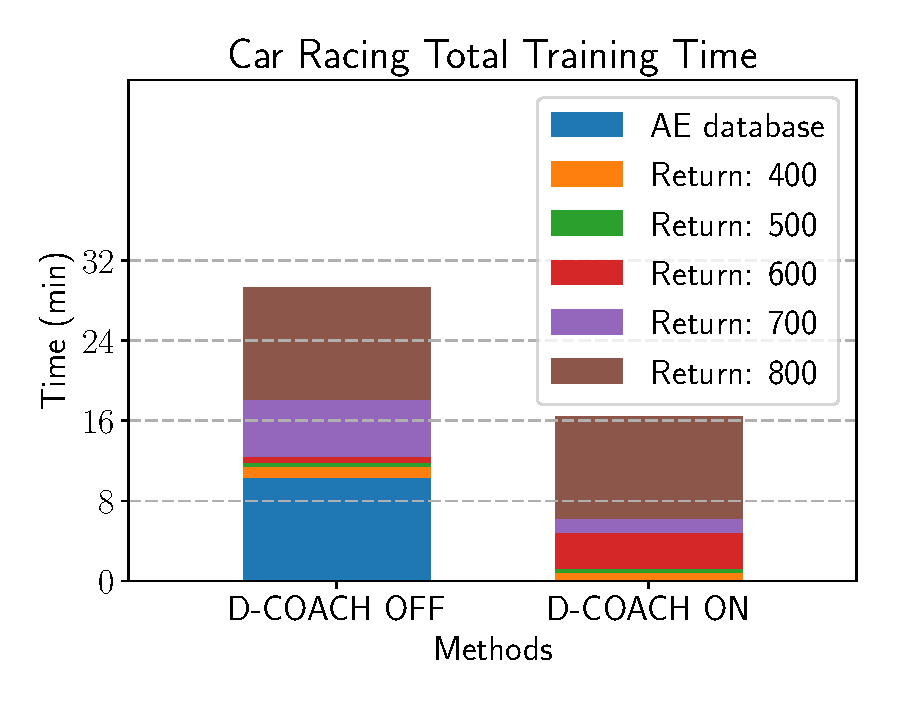
\includegraphics[width=0.5\linewidth]{imagenes/cap3/bar_car_racing_ICRA.pdf}}
\subfloat[][Duckie Racing.]{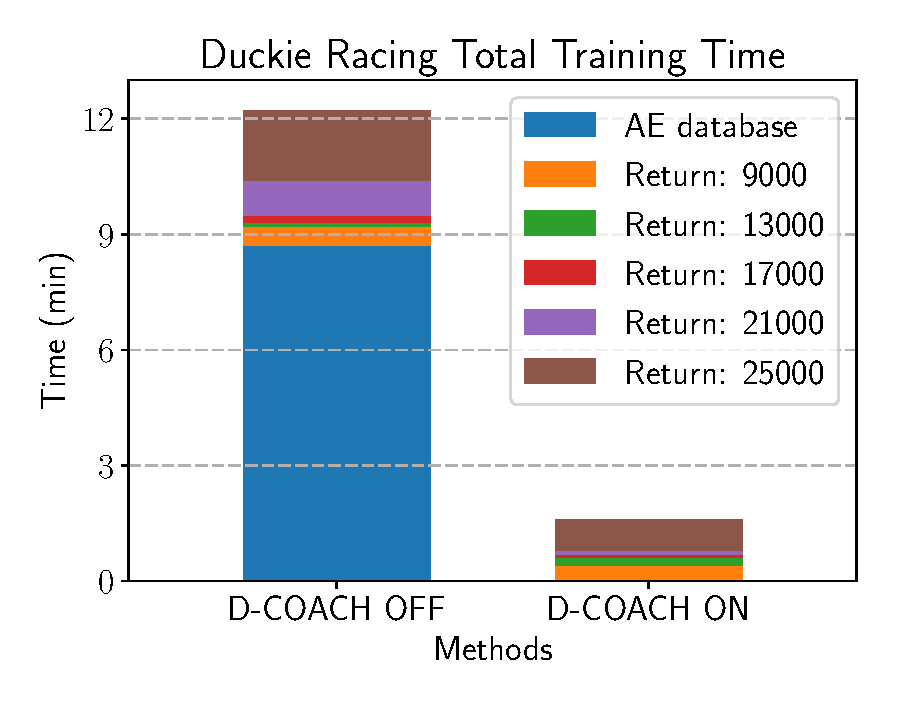
\includegraphics[width=0.5\linewidth]{imagenes/cap3/bar_duckie_ICRA.pdf}}
\caption{Comparison of the average human time dedicated to reach some levels of return.} 
\label{fig:stacked_bar} 
\end{figure}

\begin{figure}[h]
    \centering
    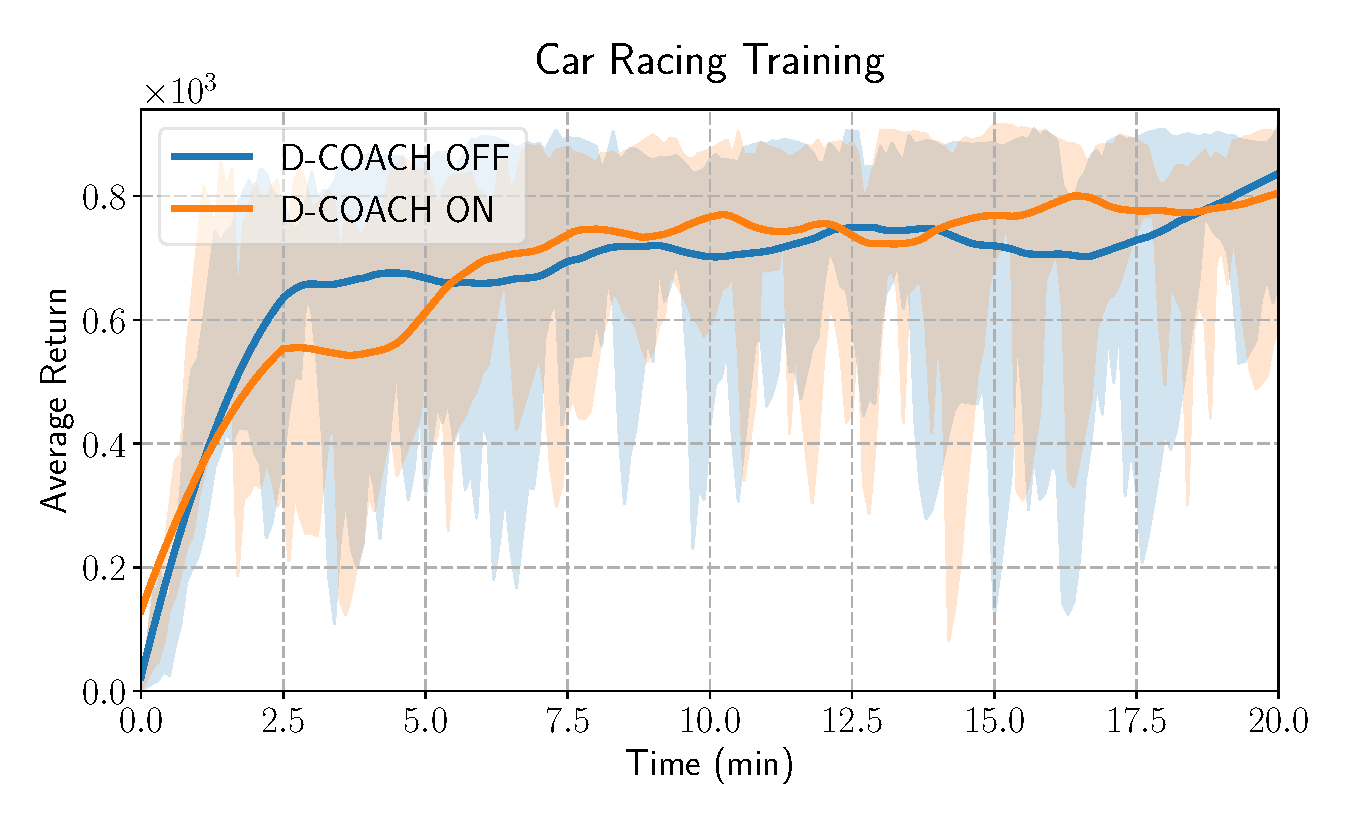
\includegraphics[width=0.9\linewidth]{imagenes/cap3/car_racing_human_teacher_ICRA.pdf}
    \caption{Results of learning with human teachers. Buffer: $K = 1000$; $b = 10$; $N = 8$.}
    \label{fig:racing_car_results}
\end{figure}

\begin{figure}[h]
    \centering
    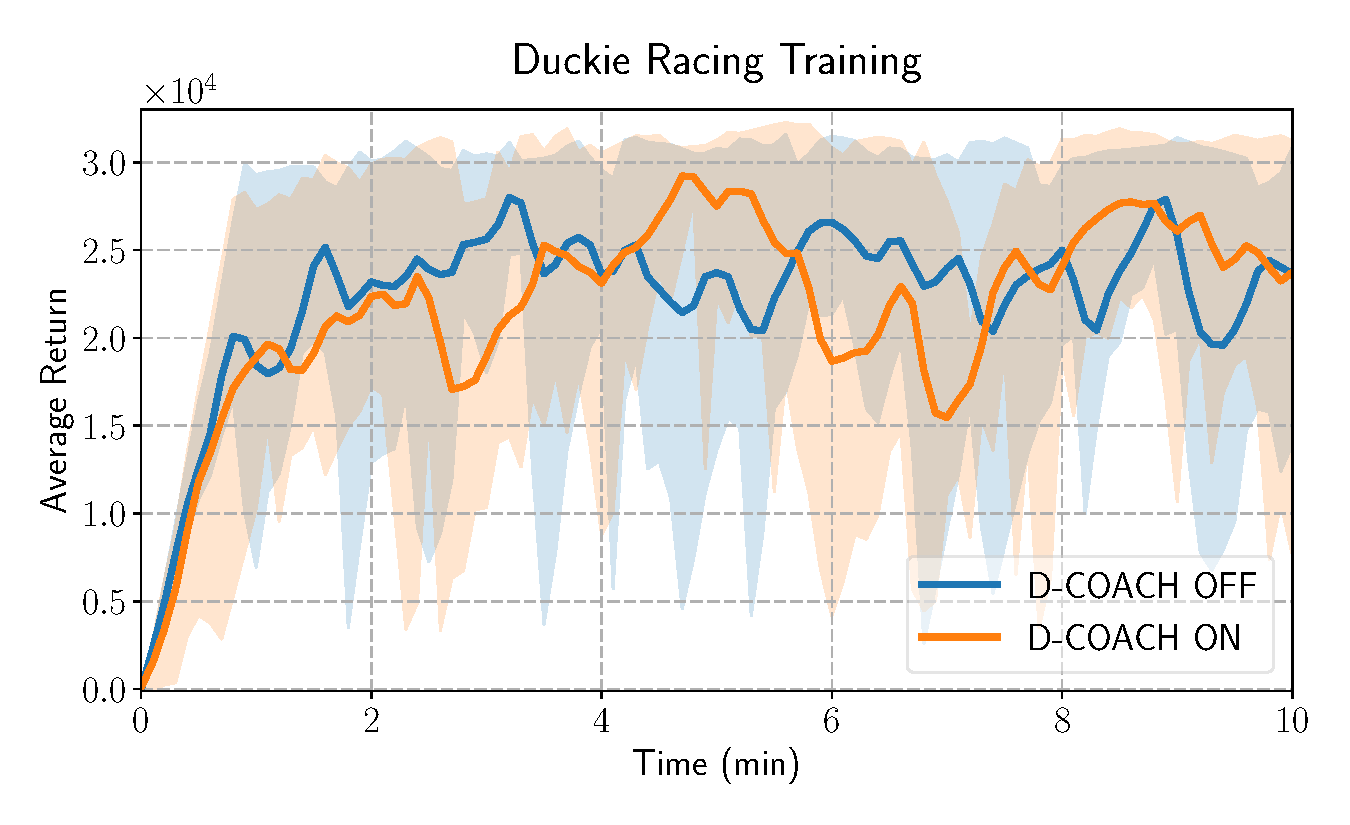
\includegraphics[width=0.9\linewidth]{imagenes/cap3/duckie_human_teacher_ICRA.pdf}
    \caption{Results of learning with human teachers. Buffer: $K = 1000$; $b = 10$; $N = 8$.}
    \label{fig:racing_car_results}
\end{figure}

\subsection{Additional validation with real systems}

Additional experiments with human teachers interacting with real robots through the enhanced D-COACH were carried out. These tests are for validating the results obtained with the previous two types of experiments, and no comparisons are presented.

A real Duckiebot was used for validating the results obtained with the simulations. An expert teacher advised the policy of Duckiebot from scratch and obtained a good policy in six minutes\footnote{https://youtu.be/Zor7z03Yfls}. 

For the reacher case, the teacher advises corrections of the position commands of the arm in the Cartesian space. The cost function for this problem is the Euclidean distance between the end-effector of the arm and the object to track, normalized with the largest possible distance within the image (distance of opposite corners). Seven training sessions of 15 minutes were run and the results are depicted in Figure \ref{fig:reacher_exp}. The link\footnote{https://youtu.be/nc2qonaKevc} shows the learning process of the reacher task during half an hour of training. Also, a pusher task training session is shown in the link\footnote{https://youtu.be/mvlIEO1WHkA}.

\begin{figure}[h]
    \centering
    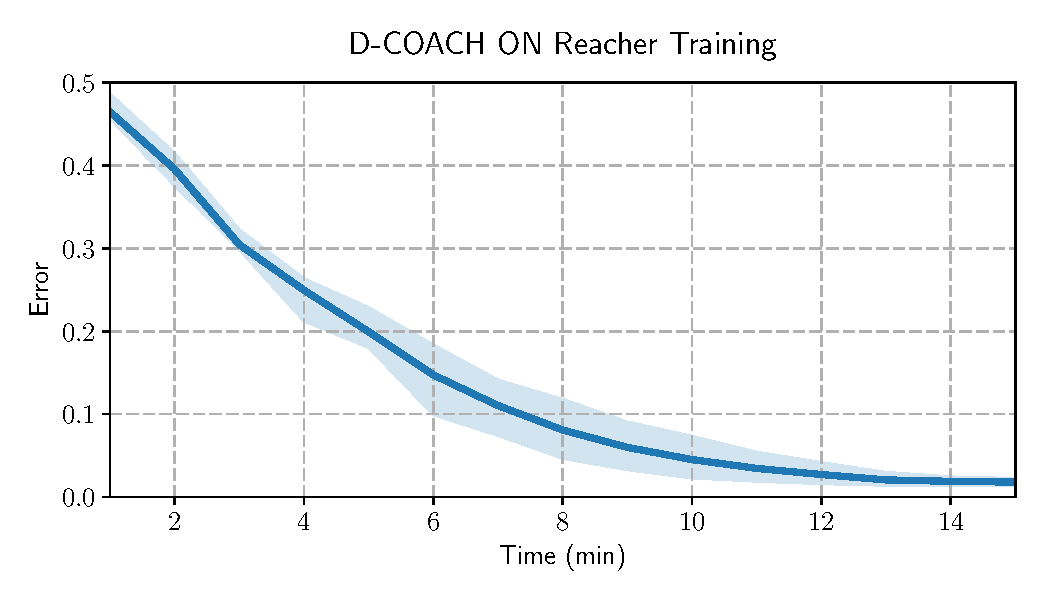
\includegraphics[width=0.9\linewidth]{imagenes/cap3/reacher_ICRA.pdf}
    \caption{Evolution of the error while learning the reacher task. }
    \label{fig:reacher_exp}
\end{figure}



\section{Low-dimensional State}


\subsection{Cart-Pole}

\section{High-dimensional State}
\subsection{Car Racing}
\subsection{Duckie Racing (simulation)}
\subsection{Duckie Racing (real robot)}
\subsection{3 DoF Arm}

\section{Low-dimensional State with Memory}
\subsection{Partially Observed Cart-Pole}

\section{High-dimensional State with Memory}
\subsection{Cart-Pole from Pixels}
\subsection{Partially Observed Car Racing}

\begin{figure}[t]
    \centering
    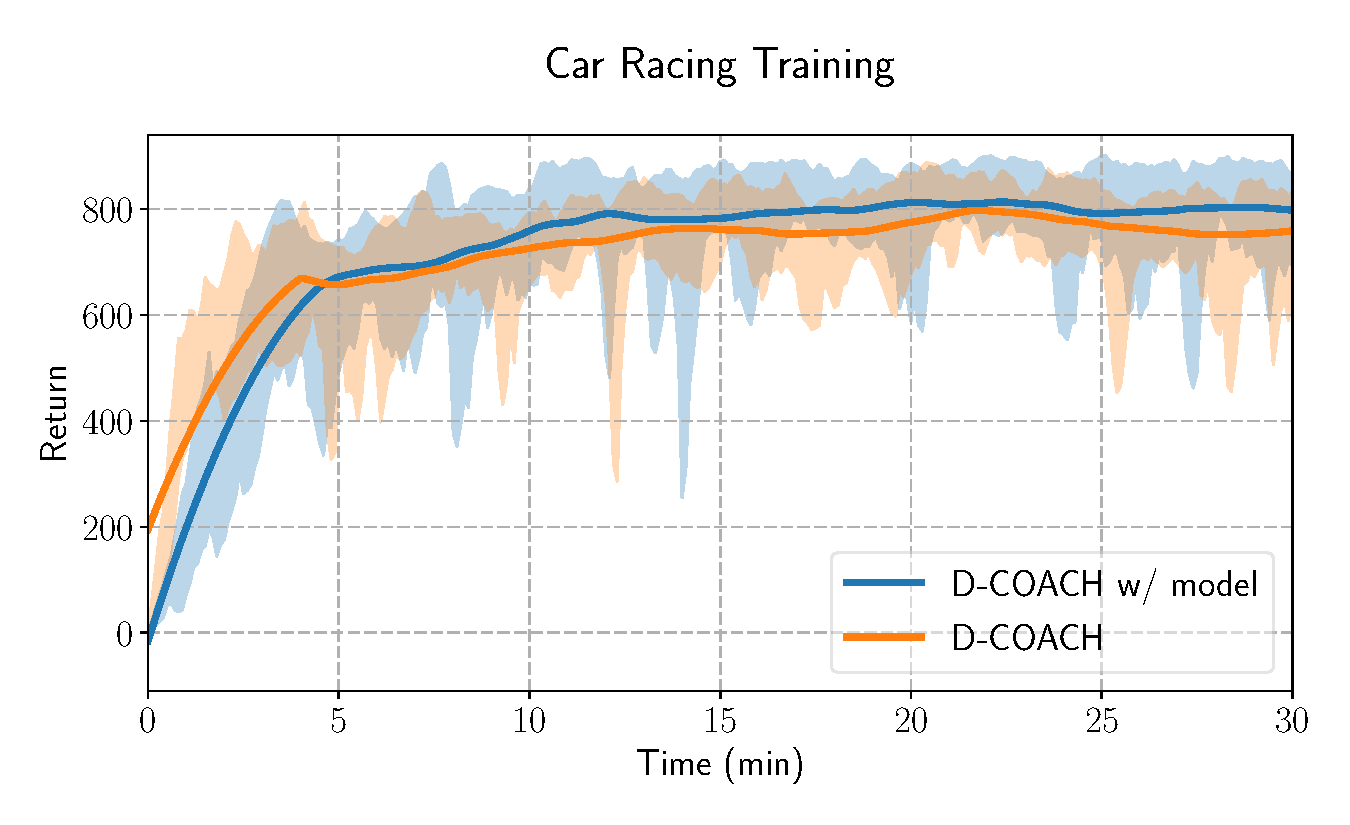
\includegraphics[width=0.9\linewidth]{imagenes/cap3/car_racing_lstm.pdf}
    \caption{Evolution of the error while learning the reacher task. }
    \label{fig:reacher_exp}
\end{figure}